\section{Exercice 2 - Détecteur de code}
\label{ex2}

Dans cet exercice nous alons modéliser le détecteur de code étudié en TD. Celui-ci lit sur une ligne de transmission série (de 1 bit) par une technique séquentielle synchrone. Un signal \textbf{Alarme} est mis à 1 dès que le code "11010" est détecté. On utilise différents signaux :
\begin{itemize}
\item BP\_0 pour l’horloge (bouton poussoir)
\item SW\_0 pour la ligne de transmission série (switch)
\item LED\_0 pour le signal Alarme
\end{itemize}

\subsection{Ports utilisés}

Au préalable, nous avons décommenté les lignes du fichier \textbf{carte\_tp.ucf} correspondant aux ports utilisés :
\textcode{Fichier : carte\_tp.ucf}
\begin{lstlisting}
NET "LED_0" LOC = "P44"  | IOSTANDARD = LVCMOS33;
NET "SW_0"  LOC = "P130" | IOSTANDARD = LVCMOS33;
NET "PB_0"  LOC = "P128" | IOSTANDARD = LVCMOS33 | CLOCK_DEDICATED_ROUTE = FALSE;
\end{lstlisting}

\subsection{VHDL}

On propose la modélisation VHDL \textbf{comportementale} ci-dessous. Chaque fausse entrée nécessite de re-entrer l'intégralité du code. Il s'agit finalement de modéliser une \textbf{machine à états}.

\vhdl
\begin{lstlisting}
entity tp2_2 is
  port(PB_0,SW_0 : in bit;
       LED_0 : out bit);	
end tp2_2;

architecture Behavioral of tp2_2 is
begin
	process(PB_0) -- Synchronisé sur chaque pression du bouton poussoir
	variable nbt : integer range 0 to 5; -- Un état pour chaque élément du code détecté + l'état où rien n'est détecté
	variable allume : bit := '0'; -- alias du signal de la LED
	begin
	if(PB_0'event and PB_0='1') then
		case nbt is
			-- A chaque pression du bouton poussoir, on vérifie que l'état du switch (1 ou 0) correspond a l'élément du code attendu (selon l'état actuel de la machine), sinon on retombe dans l'état 0 (aucun élément du code détecté)
			when 0 =>
				if(SW_0='1') then
					nbt:=1;
				end if;
			when 1 =>
				if(SW_0='1') then
					nbt:=2;
				else
					nbt:=0;
				end if;
			when 2 =>
				if(SW_0='0') then
					nbt:=3;
				else
					nbt:=0;
				end if;
			when 3 =>
				if (SW_0 ='1') then
					nbt:=4;
				else
					nbt:=0;
				end if;
			when 4 =>
				nbt:=0;
				if(SW_0='0') then -- Le code entier a été détecté
					nbt:=5;
					allume := '1';
				else
					nbt:=0;
				end if;
			when 5 => -- Une fois le code détecté (état = 5), on réinitialise tout peu importe l'état du switch
				nbt:=0;
				allume:='0';
			end case;
			LED_0<=allume; -- Affectation réelle
		end if;
	end process;				
end Behavioral;
\end{lstlisting}

\subsection{Synthèse}

\begin{figure}[!h]
   \centering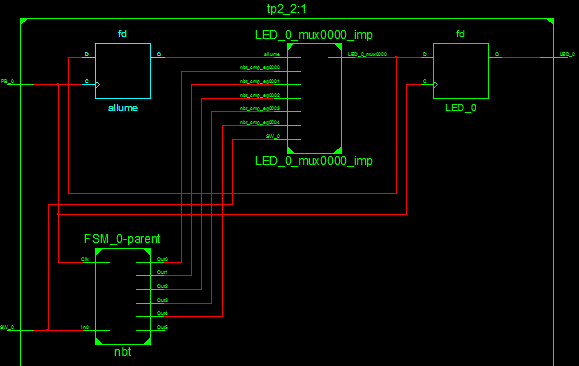
\includegraphics[width=0.74\textwidth]{files/tp2_2/rtl.png}
   \caption{Schéma RTL}
\end{figure}

On remarque que notre état (nbt) est codé sur 5 bits. Pourtant dans notre code VHDL, c'est un entier de 0 à 5, 3 bits auraient donc, à priori, été suffisants.
Au lieu d'utiliser le codage d'un entier en binaire, le synthétiseur utilise 5 bits qui activent où non un multiplexeur. Chaque bit correspond à un état.

\subsection{Simulations}

On simule notre circuit synthétisé dans ISim pour constater son bon fonctionnement.
\begin{figure}[!h]
   \centering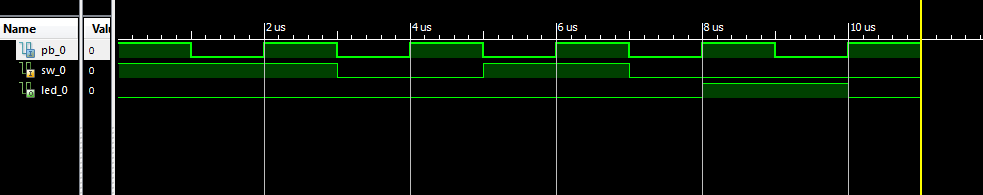
\includegraphics[width=\textwidth]{files/tp2_2/simulateur.png}
   \caption{Simulation}
\end{figure}

On fait évoluer l'entrée d'horloge à une fréquence donnée et on force les valeurs correspondant à notre code sur l'entrée ligne. On constate bien que, dès que le code est détecté, la LED s'allume (passage à 1). Elle repasse à 0 au coup d'horloge suivant, prête à détecter à nouveau le code.

\medskip

On effectue une seconde simulation pour \textbf{vérifier que lorsqu'il y a une mauvaise entrée, il y a bien réinitialisation de la machine à état}. Pour cela on compose le code avec une erreur au milieu. Si le code n'est pas détecté, c'est que l'erreur a bien été prise en compte :
\begin{figure}[!h]
   \centering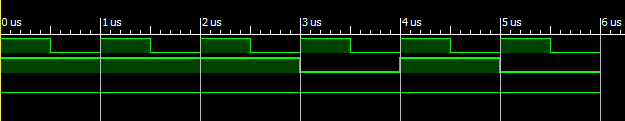
\includegraphics[width=\textwidth]{files/tp2_2/simu_erreur.png}
   \caption{Simulation}
\end{figure}

Ici, le code est correct à l'exception du 3ème '1' (à 2 $\mu$s) qui vient se glisser pour créer une erreur. On remarque que le code n'est donc pas détecté.

\bigskip

Après programmation du FPGA, on constate le bon fonctionnement pratique de notre système.

\newpage